\section{Time box 5}
\listoftodos
\subsection{Time box planning}
\begin{figure}[H]
	\begin{centering}
		\missingfigure{Updated timebox figure}
		%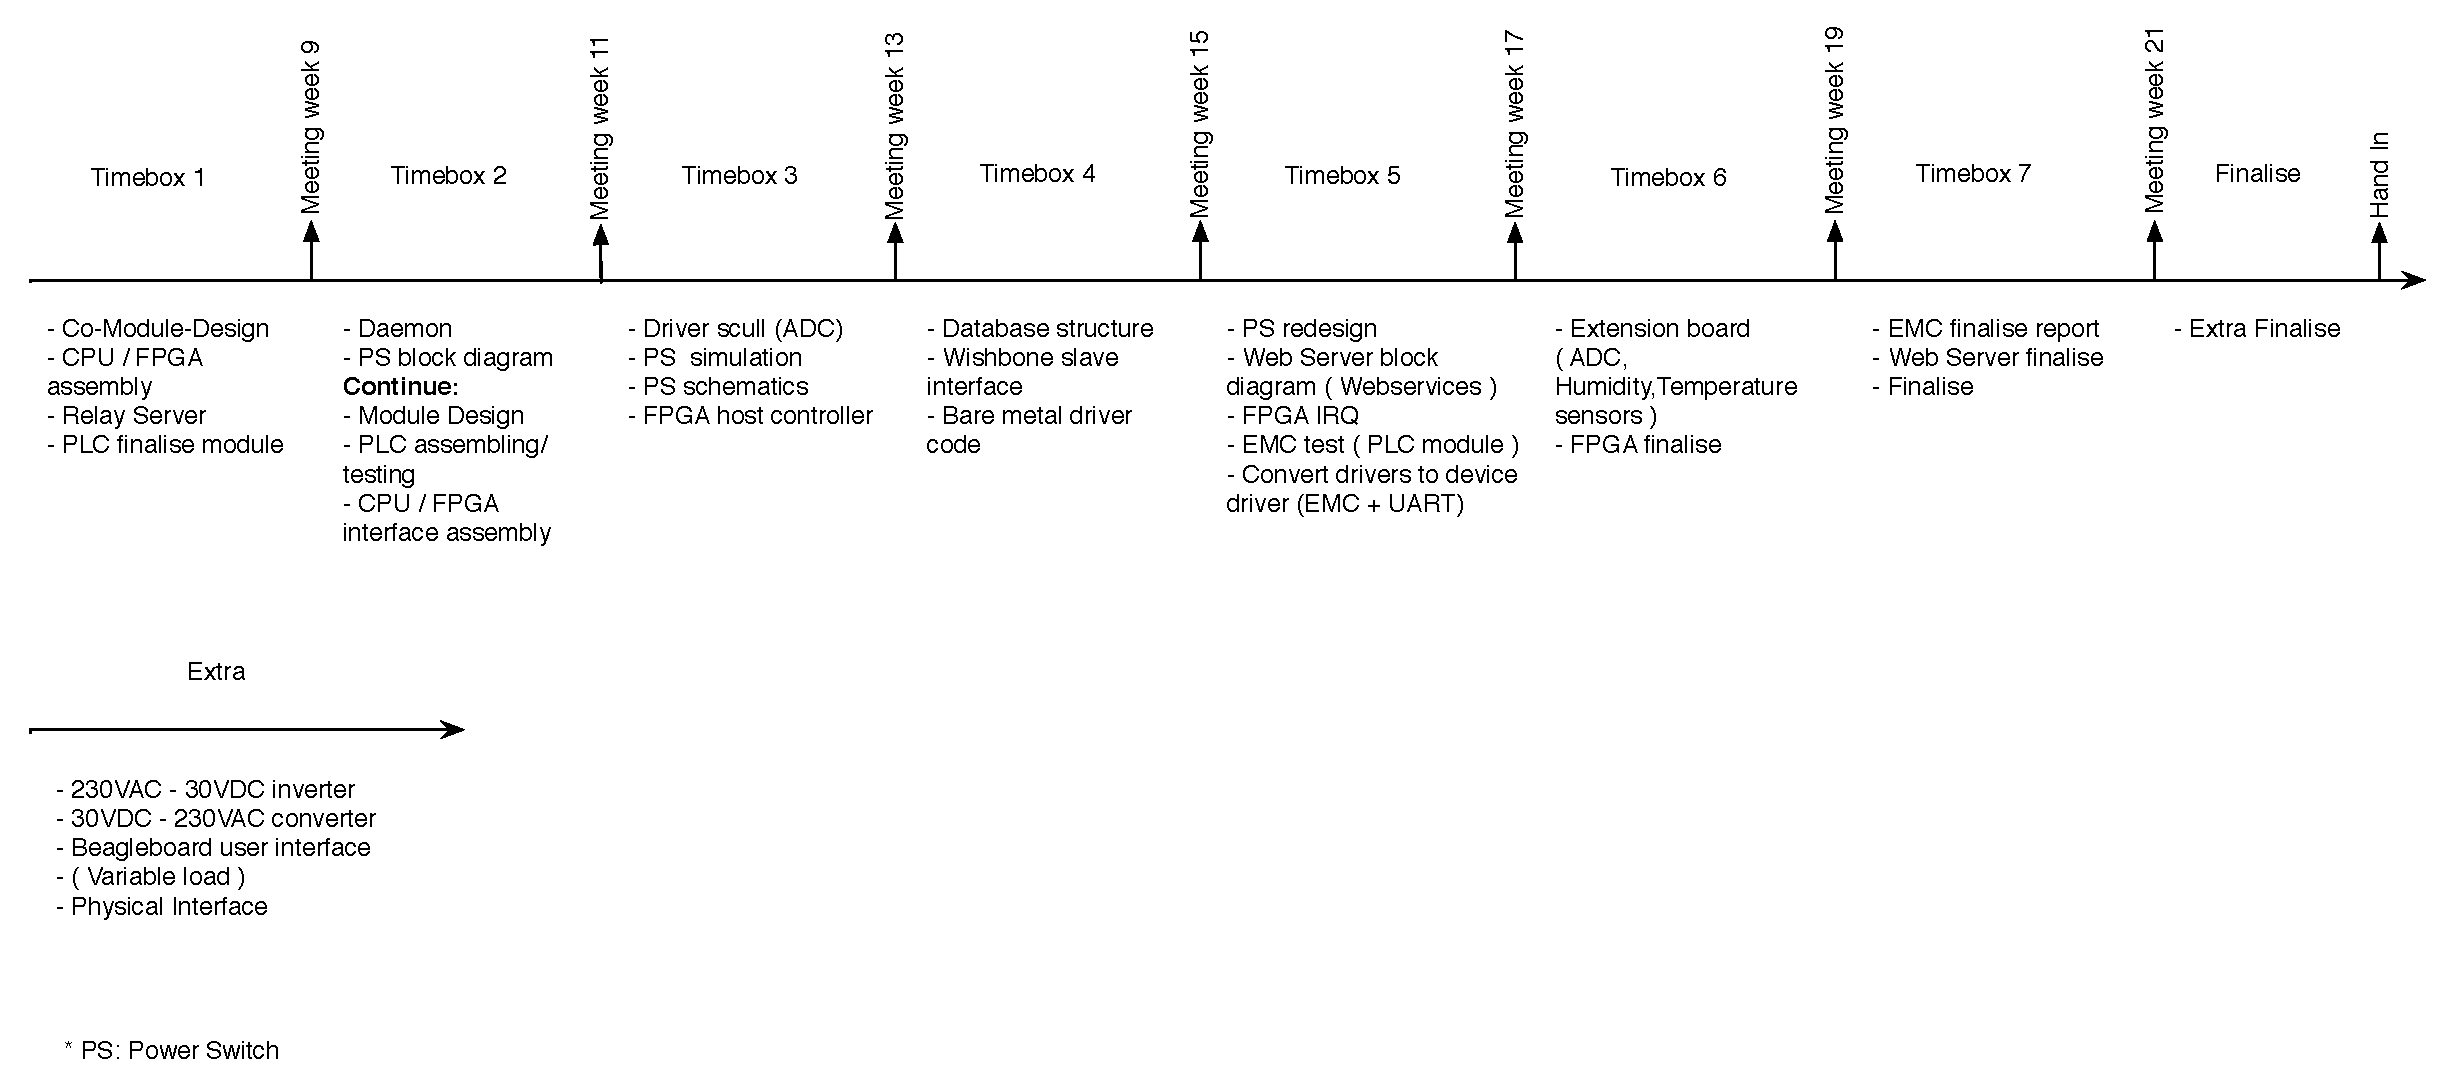
\includegraphics[width=1.0\textwidth]{images/tb_r4.pdf}
		%\caption{Updated time-box}
	\end{centering}
\end{figure}
\subsubsection{Work to be done in this time box}
\begin{itemize}
	\item Web Server
	\begin{itemize}
		\item Web Services
		\item Further improvements
	\end{itemize}
	\item Power Switch module redesign
	\begin{itemize}
		\item Improvements
		\item Simulation
		\item Redesign
	\end{itemize}
	\item Interrupt register
	\begin{itemize}
		\item Wishbone slave interface
		\item Interrupt signals
		\item Interrupt handling
	\end{itemize}
\end{itemize}
\paragraph{Description:}
\begin{description}
	\item[Something] stuff about something
	\item[Some other thing] about other thing
	\item[Interrupt register] is a block in the Spartan 6, that is allow to interrupt the ARM7 directly. The register is handling other interrupts from the Spartan 6 and tell the ARM7 where the interrupt came from.
\end{description}
\subsubsection{Time planning}
\begin{table}[H]
\centering
	\todo[inline]{Update time}
	\begin{tabular}{|l|c|c|c|c|}
		\hline
		~			& Some thing	& some other thing	& Interrupt Register\\ \hline
		Estimation	& xx			& xx				& 15				\\
		Actual		& xx			& xx				& xx				\\
		Developer	& Dennis		& Paulo			& Theis				\\
		\hline
	\end{tabular}
	\caption{Estimation and actual time used on the project}
\end{table}

\subsection{Power Switch redesign}
The prototype made in time box 3 for the power switch module didn't work as expected. New analyses and contact with Linear Technologies revealed that the IC being used (LTC...) is not the adequate component in this functionality.
%	Intro
%
%		verification specification
%		deployment specification
%
\todo{Requirements}

\subsubsection{Analysis}

\paragraph{Power switch control}
One of the problems found on the first prototype was that the LTC... device don't have a control pin to turn the MOSFETs on/off, this device will work only as an ideal diode, making it a good application for photovoltaic harvesting method.
In contact with Linear Technologies an explanation the goals for this module was given and a new device was suggested, the LTC.....

\todo{Emails with Linear Technologies}

This device as a higher and lower threshold voltage which can shut-down the device for security reasons and a shut-down pin turns on/off two MOSFET connect back to back.

\begin{figure}[H]
	\begin{centering}
		%\missingfigure{Updated timebox figure}
		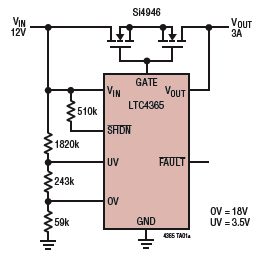
\includegraphics[width=0.5\textwidth]{images/ltc4365.png}
		\caption{LTC4365 application notes.}
	\end{centering}
\end{figure}
In this application the shut-down pin is always high which makes the device open the MOSFETS if Vin is between the under voltage and over voltage reference voltages

Linear Technologies have a simulator for them devices, the LTSpiceIV, is a free software that can be downloaded from the web site.
Is necessary to define the over and under voltage, this is found in the requirements where \todo{Get voltage range from the requirements}.

\todo{Show a bunch of calculations for the over and under voltage.}

\todo{LTC Simulations}

\todo{Full module simulation}

\paragraph{Current Sensors}

Being part of a green energy system, a current sensor is implemented in this power switch module. The measurement of current allows the system to calculate the efficiency of each module connected to its ports. The current measurements are shown to the user at the web interface.

The sensor used is a hall effect linear current sensor from Allegro, the ACS756SCA-050B, a bidirectional hall effect sensor with range from -50A to +50A. The device output an analogue signal.

\begin{figure}[H]
	\begin{centering}
		%\missingfigure{Updated timebox figure}
		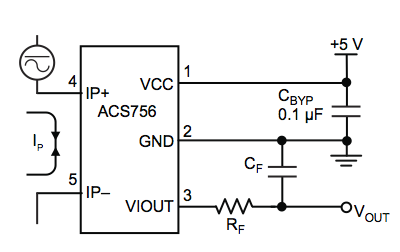
\includegraphics[width=0.5\textwidth]{images/current_sensor.png}
		\caption{ACS756SCA Typical aplication}
	\end{centering}
\end{figure}
%
%	Analysis
%
%                Refactored block diagram
%                Refactored class diagram
%                Detailed use cases
%                User interface specification
%                System interface specification
%                Dimensioning specification 
%
\subsubsection{Design}
%
%	Design
%
%                UML/SysML deployment view(s)
%                Mechanical specifications and dimensioning
%                HW module specification per block
%                UML SW deployment view
%                Class specification
%                Refactored class diagram
%                Use case scenarios specifications
%                Sequence diagrams
%
\subsubsection{Implementation}
%
%	Implementation
%
%                Mechanical drawings with details explained
%                Electronic diagrams with details explained
%                Source code with details explained
%                Description of integration 
\subsubsection{Verification}
%
%	Verification
%
%                Module tests
%                Integration tests
%                Acceptance test 


\subsection{Web Server - Paulo}

%	Intro
%
%		verification specification
%		deployment specification
%
\subsubsection{Analysis}
%
%	Analysis
%
%                Refactored block diagram
%                Refactored class diagram
%                Detailed use cases
%                User interface specification
%                System interface specification
%                Dimensioning specification 
%
\subsubsection{Design}
%
%	Design
%
%                UML/SysML deployment view(s)
%                Mechanical specifications and dimensioning
%                HW module specification per block
%                UML SW deployment view
%                Class specification
%                Refactored class diagram
%                Use case scenarios specifications
%                Sequence diagrams
%
\subsubsection{Implementation}
%
%	Implementation
%
%                Mechanical drawings with details explained
%                Electronic diagrams with details explained
%                Source code with details explained
%                Description of integration 
\subsubsection{Verification}
%
%	Verification
%
%                Module tests
%                Integration tests
%                Acceptance test 



\subsection{Interrupt register - Theis}
The interrupt register is made to tune performance by limiting the number of read statements the ARM7 is doing, in order to read from the Spartan 6. The interrupt register is not by itself fulfilling any requirements, but it is tuning the following: \textit{NF-1.5}\footnote{Requirement is found in table 3.2 in EPRO 3 project energy-hub} and \textit{B-3}\footnote{Requirement is found in table 3.4 in EPRO 3 project energy-hub}
\begin{table}[H]
\centering
	\begin{tabular}{|p{1.2cm}|p{2.3cm}|p{6cm}|p{6cm}|}
	\hline
	ID		& Requirement		& Description																& Comments\\\hline
	NF-1.5	& HW Interface		& 1 start button for the hub. 10 buttons to each start a module.			& It is only reading if the buttons state changes\\\hline
	B-3		& Errors			& Humidity and Temperature sensor will be placed inside the system housing	& The Spartan 6 interrupts if one of the following is happening\\\hline
	B-3.1	& Humidity			& If the humidity is above the maximum level 70\%, the system shuts down	& ARM7 only read on interrupt\\\hline
	B-3.2	& Temperature High	& If the temperature is higher than 55 degrees, the system shuts down		& ARM7 only read on interrupt\\\hline
	B-3.3	& Temperature Low	& If the temperature is below 0 degrees, the system shuts down				& ARM7 only read on interrupt\\\hline
	\end{tabular}
\end{table}
%			Intro
%					verification specification
%					deployment specification
\subsubsection{Analysis}
The purpose of the interrupt register is to limiting the number of readings the ARM7 is making from the Spartan 6. There is one interrupt pin routed from the AMR7 to the Spartan 6, but there is two blocks in the Spartan 6 that makes data for the ARM7. These blocks are the switch input block and the analog to digital converter\footnote{ADC} block. One way to use the interrupt is to allow the switch block to interrupt when a user interact with the system, and then read the ADC with a specific time interval. But to avoid to many unnecessary readings of the ADC, the interrupt register is the only block that is allow to interrupt the ARM7, the interrupt register gets interrupt signals from the ADC and the switch blocks, the register is arranging the interrupt, and when the ARM7 is interrupted, it reads data from the register to find out which block it should read.
\begin{figure}[H]
	\begin{centering}
		%\missingfigure{Updated timebox figure}
		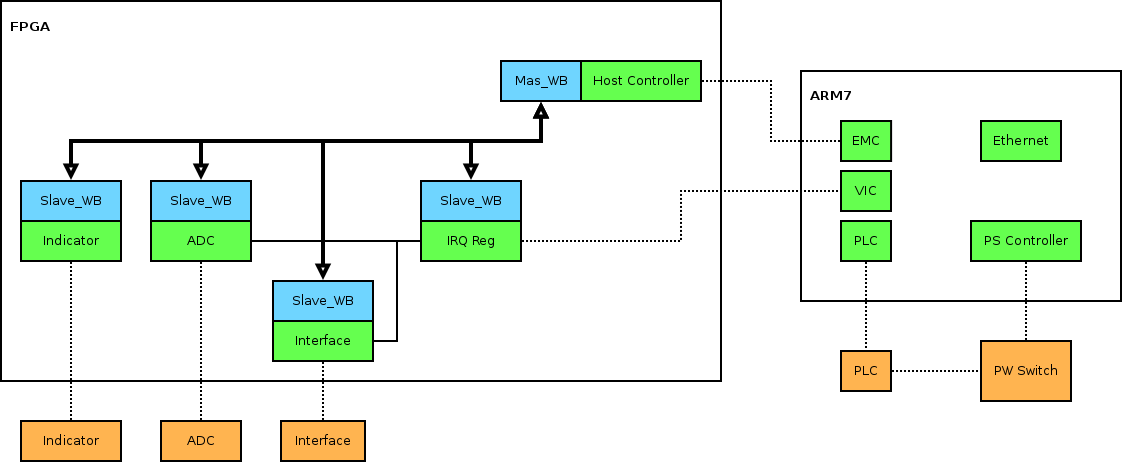
\includegraphics[width=1.0\textwidth]{images/tb5_modules_design.png}
		\caption{Module design with IRQ register}
	\end{centering}
\end{figure}
When a block sends an interrupt to the IRQ\footnote{Interrupt Request} register, it locates the interrupt and put the address to the block on to a FIFO\footnote{First In First Out}, and sends an interrupt to the ARM7, then the AMR7 read the FIFO to get the address on the interrupting block, in that way the ARM7 knows where to read next.
%			Analysis
%
%                Refactored block diagram
%                Refactored class diagram
%                Detailed use cases
%                User interface specification
%                System interface specification
%                Dimensioning specification 
%
\subsubsection{Design}
The purpose of the interrupt register is to make interrupt functionality on several block with only one interrupt pin to the ARM7. The interrupt register shall be optimized to wishbone use. The interrupt register without wishbone has to inputs, a vector of size N\footnote{N = number of blocks that is allow to interrupt} and an array that is N bit high and AddrRange\footnote{Wishbone address range} bit wide. The output is the IRQ pin to the ARM7 and a data vector equal to the wishbone data width. This is shown in the figure below.
\begin{figure}[H]
	\begin{centering}
		%\missingfigure{Updated timebox figure}
		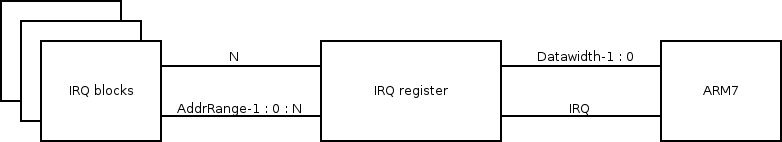
\includegraphics[width=1.0\textwidth]{images/tb5_irq_reg_nowb.png}
		\caption{IRQ register without wishbone}
	\end{centering}
\end{figure}
When a block needs to make an interrupt, it puts the wishbone address onto the input array to the IRQ register, and then sets the interrupt output high to tell the IRQ register that there is a valid address that needs to be read. The IRQ register save the address and interrupt the ARM7. When an interrupt occurs on the ARM7, it read the IRQ register to get the address that it shall read next, in this way it takes two wishbone read cycles for the ARM7 to get the right data, but the ARM7 is only reading if the Spartan 6 have valid data to read, instead of make reading with specific interval. The IRQ register save the interrupt in a FIFO in case interrupt is made faster than the ARM7 can read.\\
\paragraph{Interrupt output}
The interrupt output is set every time the FIFO gets data and the earlier state was empty. This mean that the interrupt is set low when the FIFO gets the first data, if the FIFO gets more data and have not been emptied the IRQ is set high, and first set low again when the FIFO has been emptied.
\paragraph{Data output}
The data output is equal to the wishbone data width, in this case it is 16 bit, and the address is 7 bit. The seven lowest data bits is used for the address to the block that sends the interrupt, the rest of the bits is used to tell the ARM7 how many spaces that is filled in the FIFO. In this way the ARM7 know when it is reading the last interrupt, and shall stop reading.
\begin{figure}[H]
	\begin{centering}
		%\missingfigure{Updated timebox figure}
		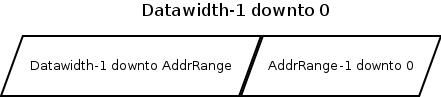
\includegraphics[width=0.55\textwidth]{images/tb5_irq_reg_data_o.png}
		\caption{IRQ register data output}
	\end{centering}
\end{figure}
%        Design
%
%                UML/SysML deployment view(s)
%                Mechanical specifications and dimensioning
%                HW module specification per block
%                UML SW deployment view
%                Class specification
%                Refactored class diagram½
%                Use case scenarios specifications
%                Sequence diagrams
%
\subsubsection{Implementation}
%        Implementation
%
%                Mechanical drawings with details explained
%                Electronic diagrams with details explained
%                Source code with details explained
%                Description of integration 
%
\subsubsection{Verification}
%        Verification
%
%                Module tests
%                Integration tests
%                Acceptance test
\subsubsection{Conclusion}



\subsection{Deployment}
\paragraph{Something}
	%which versions of the prototype the customer will get
	%with what functionality.	
\paragraph{Some other thing}
	%which versions of the prototype the customer will get
	%with what functionality.
\paragraph{Interrupt register}
	%which versions of the prototype the customer will get
	%with what functionality.